\chapter{Versuch 1 - Bestimmung der Tonhöhe eines akustischen Signals}
\label{chap:VERSUCH_1}


\section{Fragestellung, Messprinzip, Aufbau, Messmittel}
\label{chap:VERSUCH_1_FRAGESTELLUNG}

\subsection*{Fragestellung}
	In diesem Versuch geht es darum einen einzelnen Ton eines Musikinstruments mit einem Mikrofon aufzunehmen.
Das daraus resultierende Signal soll dann in sein Spektrum zerlegt und dargestellt werden.
Dadurch soll ein praktisches Verständnis für die Messung von Tonsignalen und der Fourieranalyse vermittelt werden.
	
\subsection*{Messprinzip}
Die Fourieranalyse ist ein essenzielle Methoden für die Signalverarbeitung. Sie erlaubt es die Grundfrequenz sowie die Obertöne einer Schwingung zu ermitteln.

\subsection*{Aufbau}


\includegraphics[scale=0.4]{media/Versuchaufbau.png}
\label{Abb:Aufbau}


\subsection*{Messmittel}
\begin{itemize}
	\item Mikrophon
	\item Klanguelle (Klarinette)
\end{itemize}

\section{Messwerte}
\label{chap:VERSUCH_1_MESSWERTE}

Zwei Schwinungen, aus den späteren abschnitten (die ersten 50.000 Werte wurden übersprungen, weil das Signal zu verworren war)
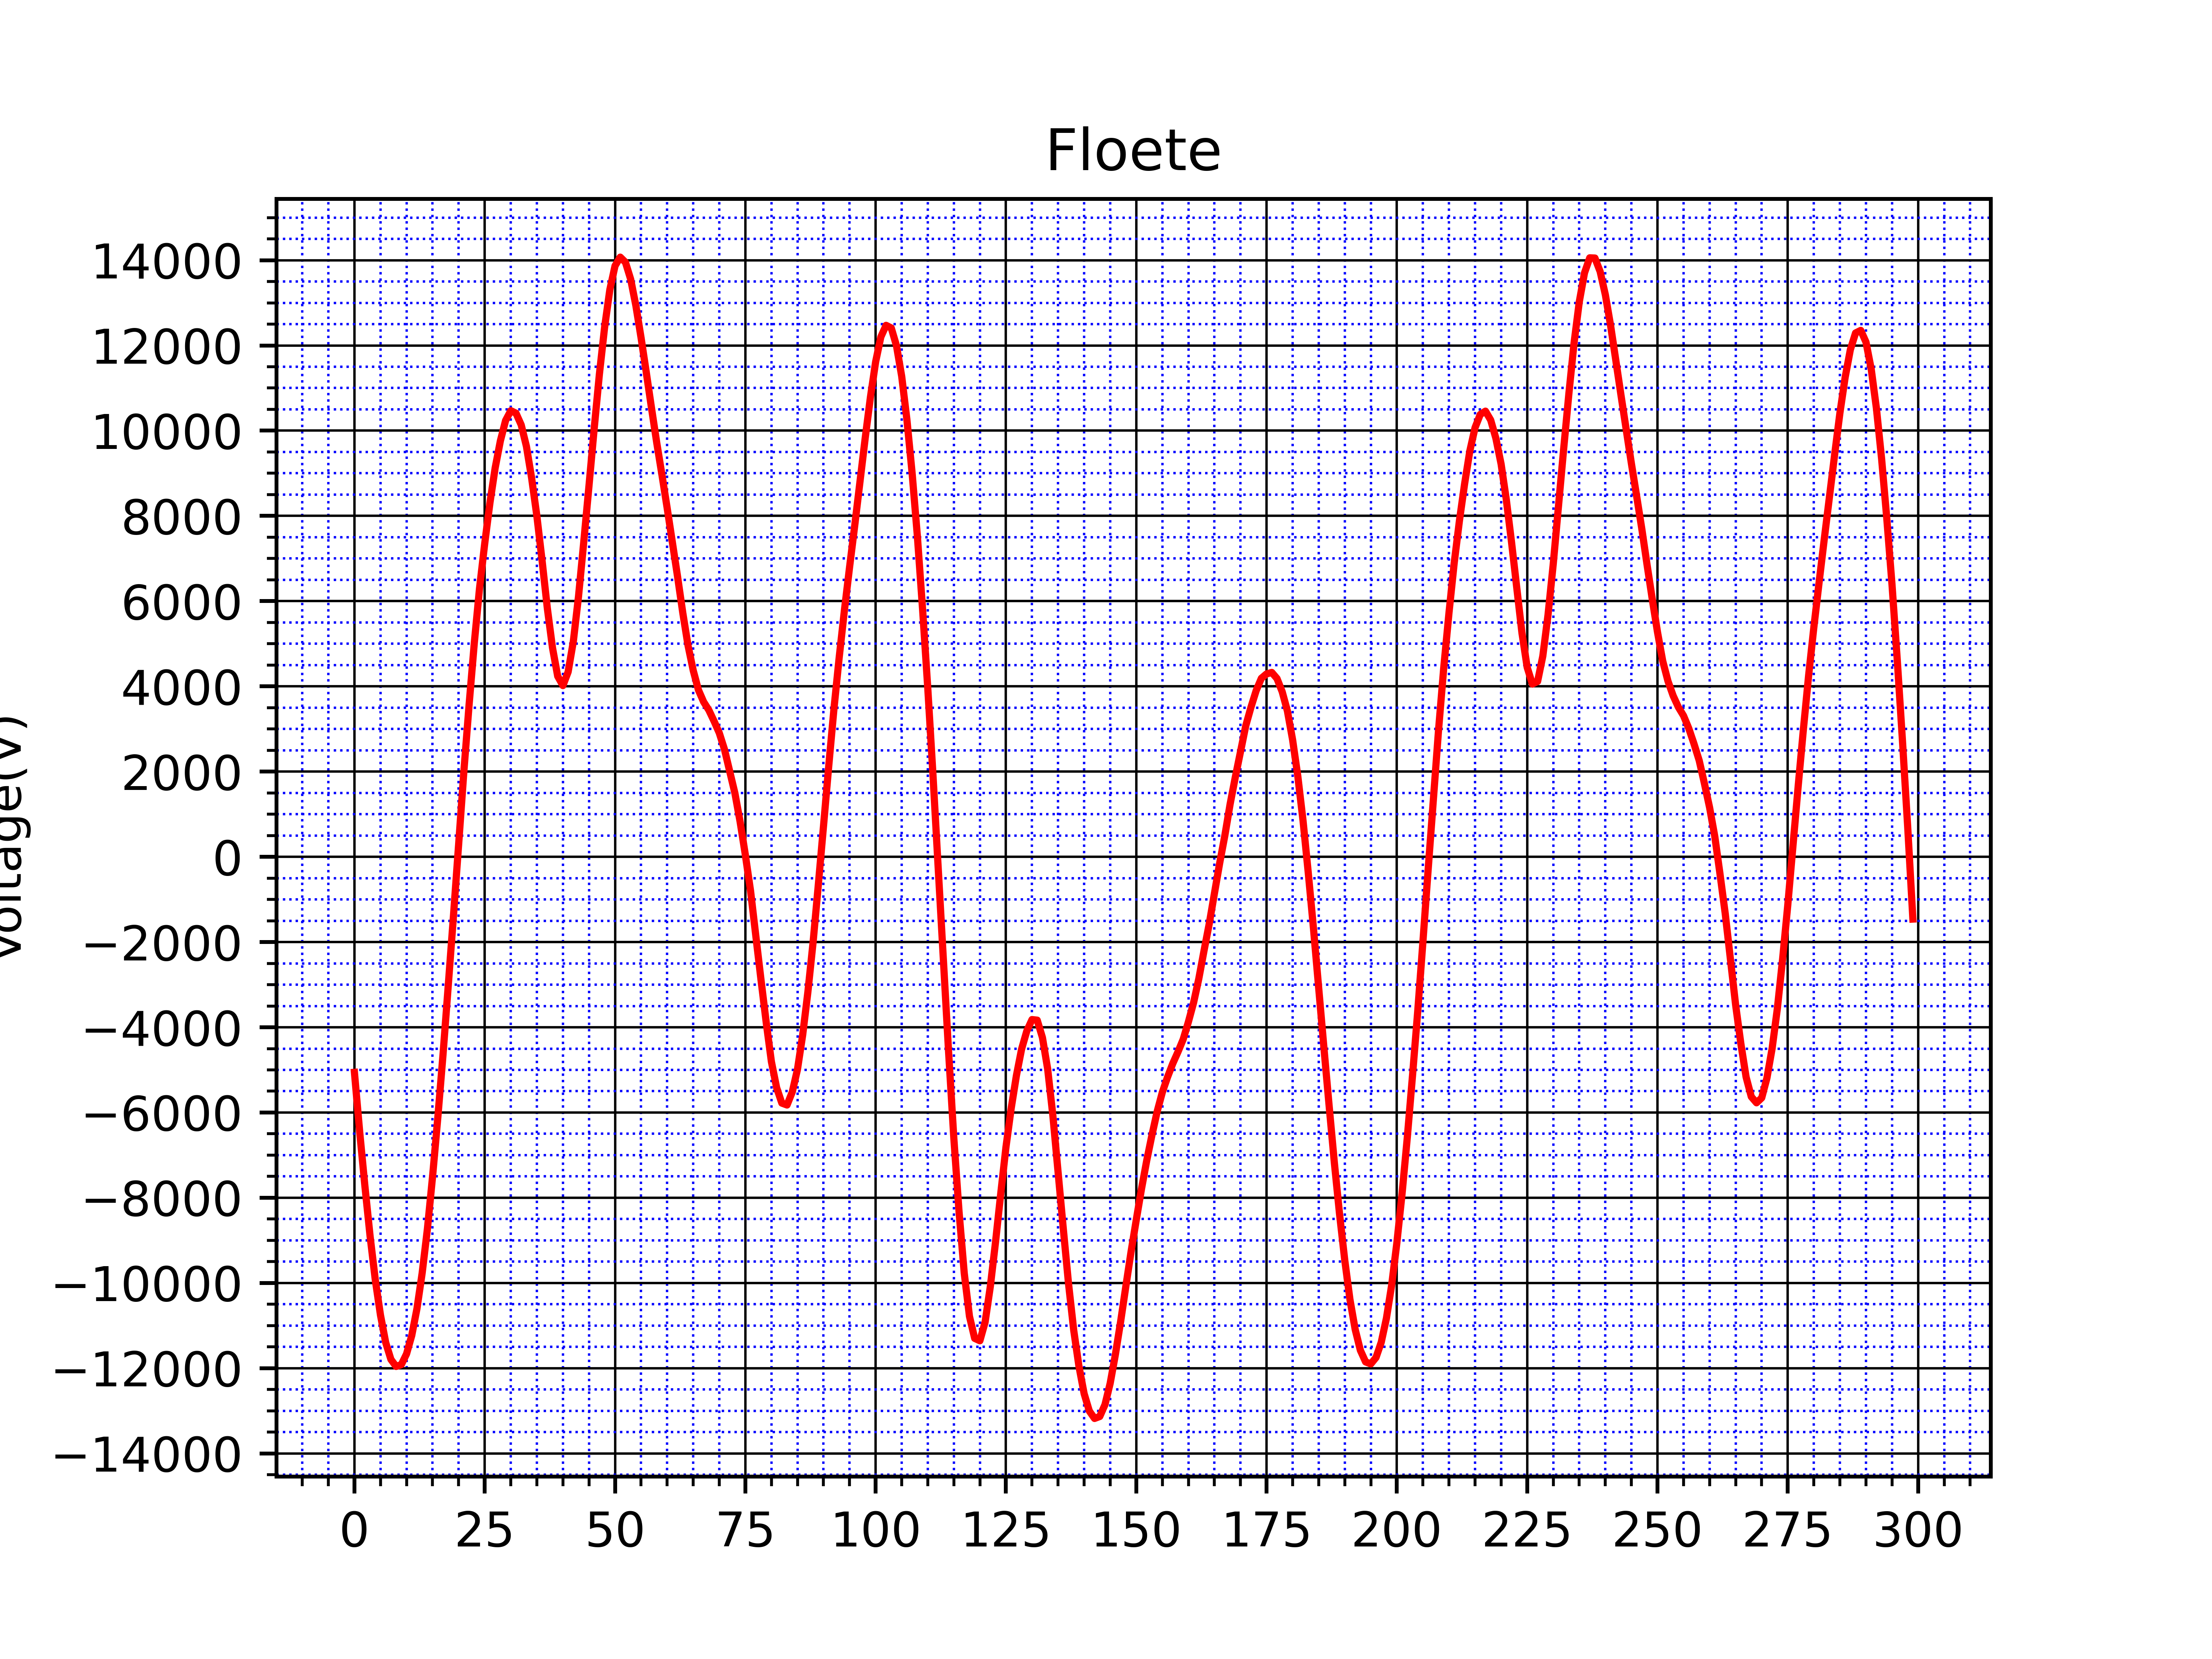
\includegraphics[scale=0.05]{media/Signal_Raster.png}

Die Werte auf der X-Achste stehen hierbei für Abtastpunke über die Zeit und sind daher einheitslos.

\section{Auswertung}
\label{chap:VERSUCH_1_AUSWERTUNG}

Vor Beginn der eigentlichen Auswertung werden erst  mal die Randdaten festgelegt. Das Signal wurde mittels des Beispielprogramms audioSample.py aufgenommen und abgespeichert. Dabei hat das Programm über einen Gesamtzeitraum von 225280 Frames gemessen und in dieser wurden 44100 Frames die Sekunde gemessen.
Das bedeutet die \textbf{Abtastfrequenz} war 44100 Hz.
Daraus lässt sich auch die Messdauer berechnen:
\begin{equation}
	M = \frac{N}{at} = \frac{225280}{44100 Hz} = 5,1084 s
\end{equation}
\begin{itemize}
	\item M = Signallänge
	\item N = Anzahl Framse = 225280
	\item at = 
\end{itemize}

, daraus ergibt sich eine Messdauer von insgesamt 5,1084 s.
Die Framezeit und somit das Abtastintervall ist 0,000022676 s oder 0,022676 ms.
Abtastfrequenz ist 441000 Hz


Zunächst werden die Grundperiode und die Grundfrequenz des Signals anhand des Plots ermittelt:

Grundperiode: Zeitliche dauer bis sich die Schwingung wiederholt. Sie muss folglich aus den Plot abgelesen werden:
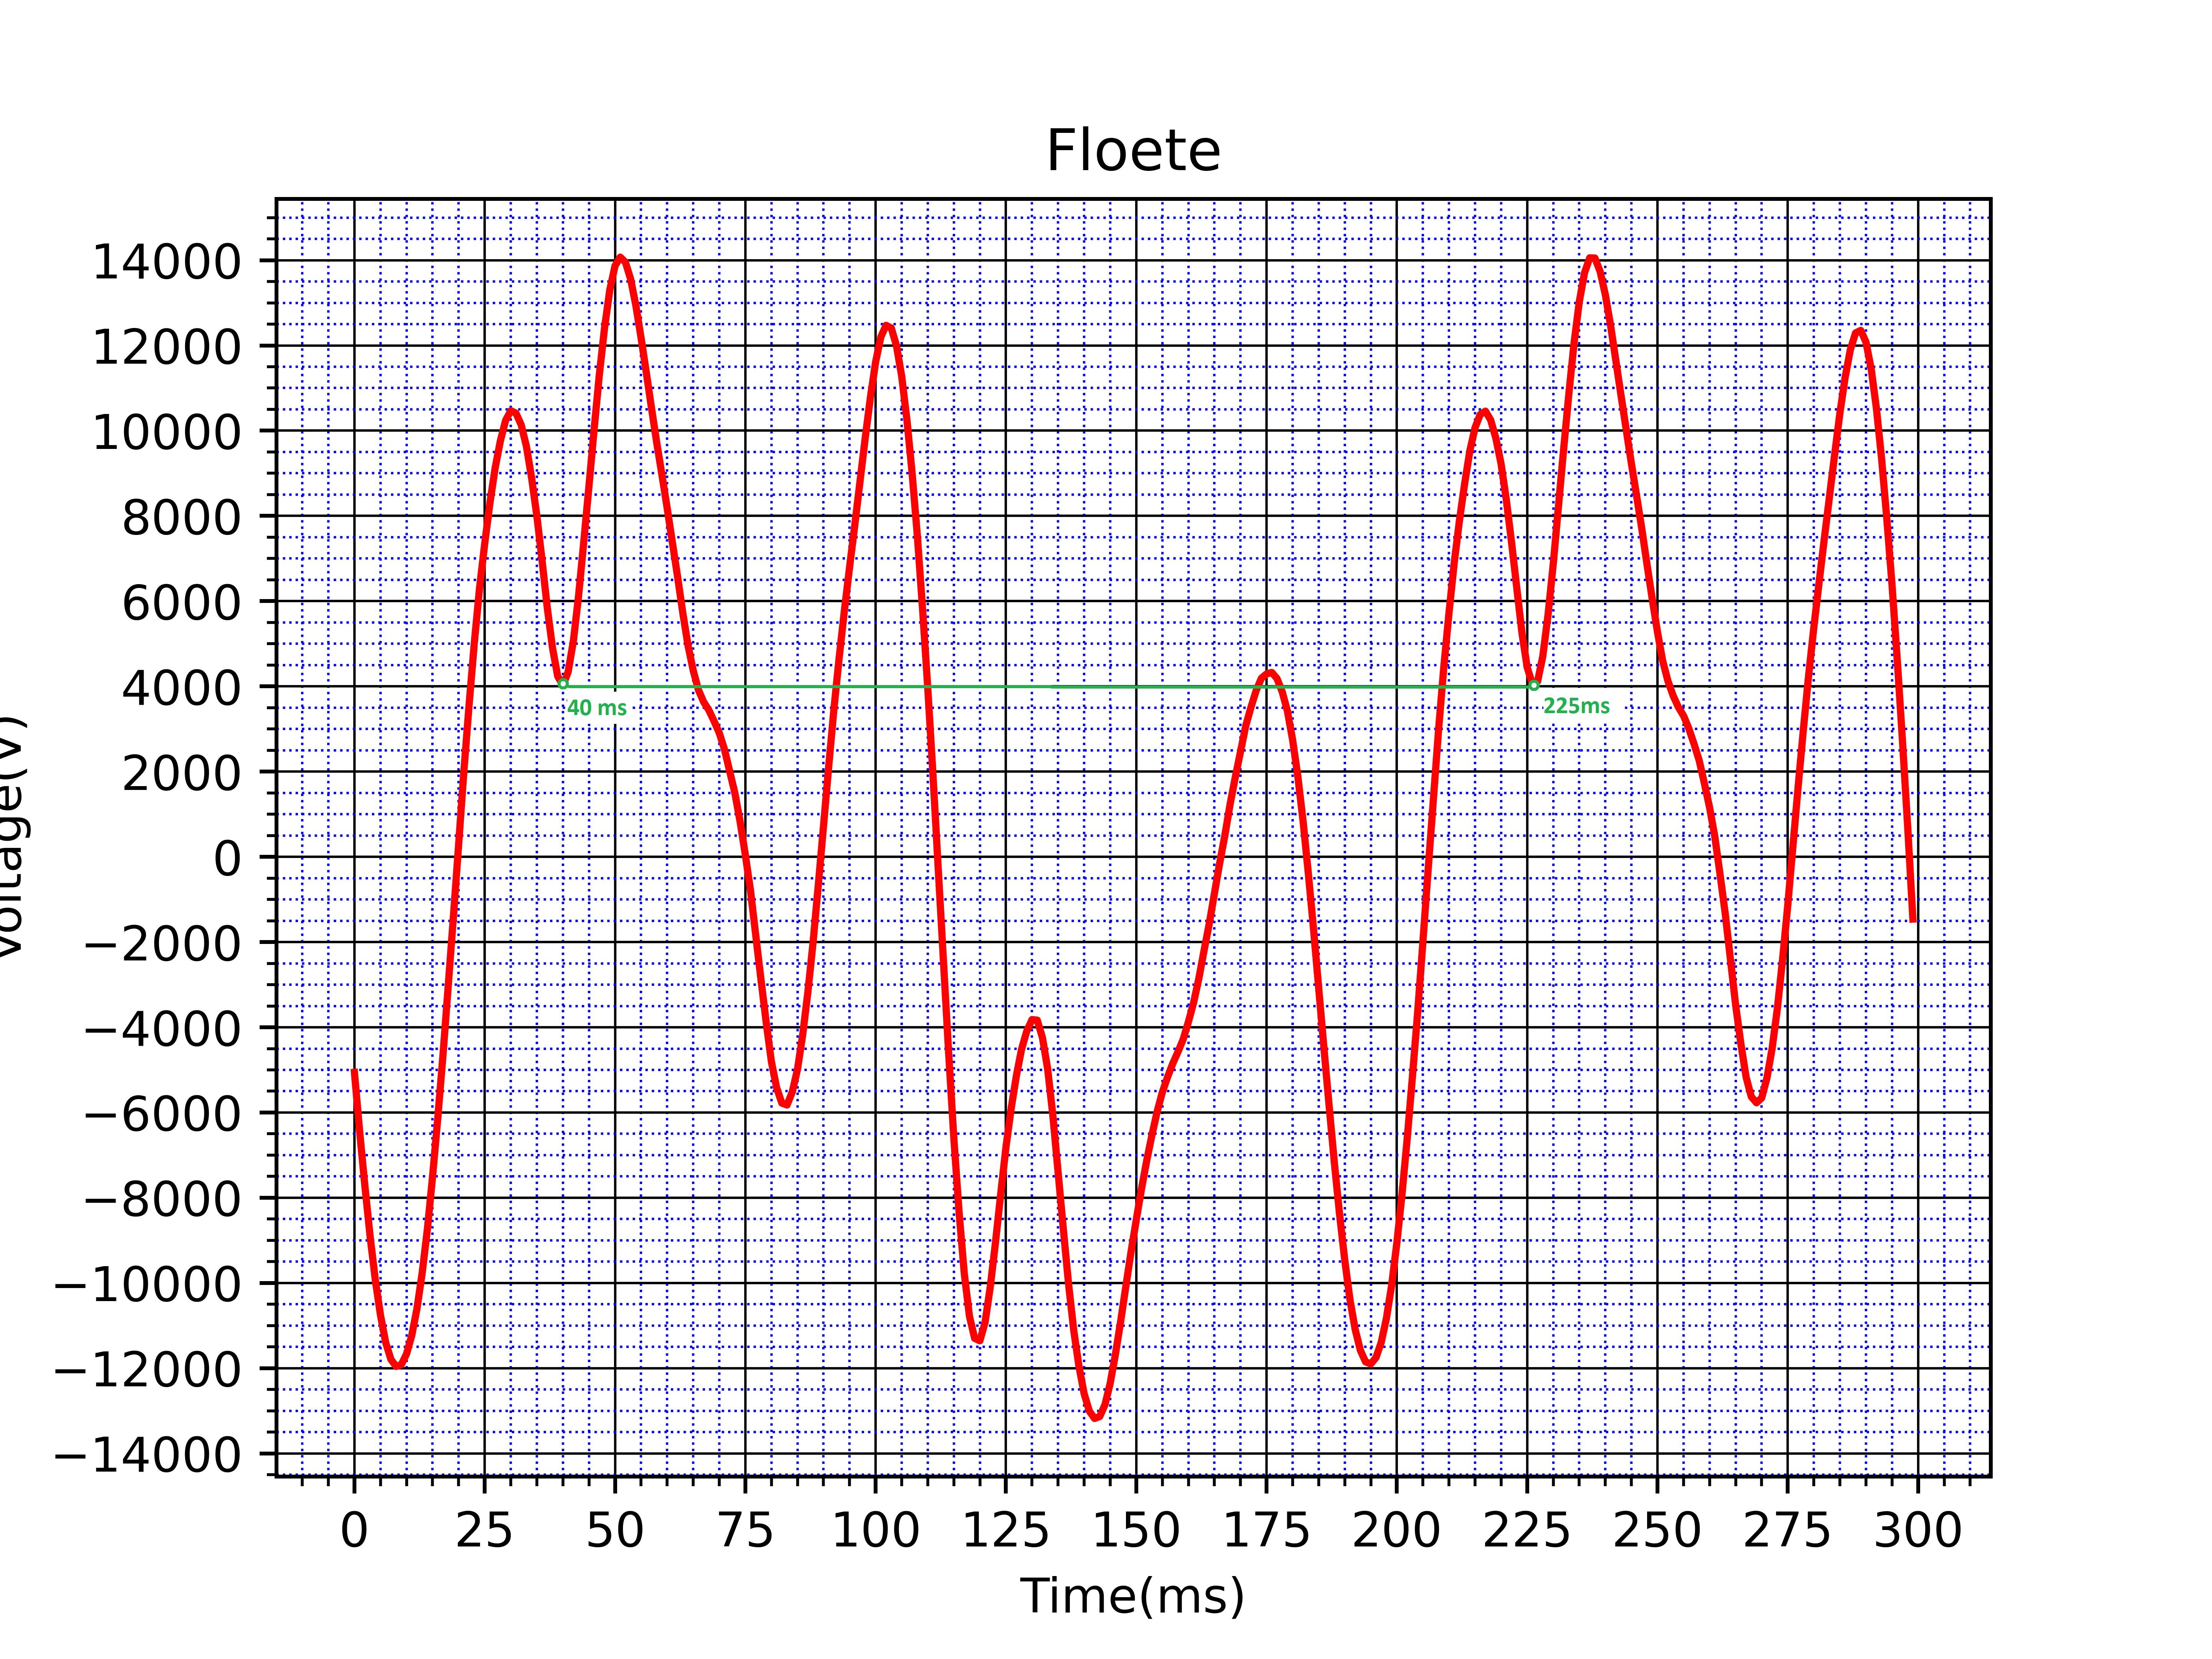
\includegraphics[scale=0.05]{media/Signal_Raster_Periode.png}

An der Graphik lässt sich erkennen das $ Grundperiode = 225 - 40 = 185 $ ist.
Dabei sei zu erwähnen das die 185 für die Anzahl von Abtastpunkten steht über die eine Periode dauert.

Die Frequenz ergibt sich aus:
\begin{equation}
	f = n / t
\end{equation}
\begin{itemize}
	\item f = Frequenz in Hz
	\item n = Anzahl Schwingungen
	\item t = Gemessener Zeitraum in s
\end{itemize}




nun wird die 



\section{Interpretation}
\label{chap:VERSUCH_1_INTERPRETATION}